\documentclass[pdf,table]{beamer}
\usepackage{graphicx,hyperref,pdfpages}
\usepackage{tikz}
\usepackage{textpos}
\usepackage{longtable}
\usepackage{listings}
\usepackage{colortbl}
%\usepackage[table]{xcolor}
%\usepackage{multirow}
\usetikzlibrary{arrows}
\usetikzlibrary{positioning,chains,fit,shapes,calc}
\usetikzlibrary{mindmap}

%defin colours
\definecolor{codegreen}{rgb}{0,0.6,0}
\definecolor{codegray}{rgb}{0.5,0.5,0.5}
\definecolor{codepurple}{rgb}{0.58,0,0.82}
\definecolor{backcolour}{rgb}{0.95,0.95,0.92}
\definecolor{delim}{rgb}{20,105,176}



\lstdefinelanguage{CTO}{
	keywords={abstract, asset, by, concept, default, enum, event, identified, Integer, o, participant, String, transaction },
	comment=[l]{//},
	comment=[s]{/*}{*/},
	string=[b]",
	sensitive=true,
}

\lstdefinelanguage{ACL}{
	keywords={transaction,condition,rule,description,participant,operation,resource,action,ALLOW,READ,ALL,CREATE,UPDATE,DELETE,ANY,DENY},
	comment=[l]{//},
	comment=[s]{/*}{*/},
	string=[b]",
	sensitive=true,
}

%define Javascript language
\lstdefinelanguage{JavaScript}{
keywords={typeof, new, true, false, catch, function, return, null, catch, switch, var, if, in, while, do, else, case, break},
keywordstyle=\color{blue}\bfseries,
ndkeywords={class, export, boolean, throw, implements, import, this},
ndkeywordstyle=\color{darkgray}\bfseries,
identifierstyle=\color{black},
sensitive=false,
comment=[l]{//},
morecomment=[s]{/*}{*/},
commentstyle=\color{purple}\ttfamily,
stringstyle=\color{red}\ttfamily,
morestring=[b]',
morestring=[b]"
}
%define json language
\colorlet{punct}{red!60!black}
\definecolor{background}{HTML}{EEEEEE}
\definecolor{delimiter}{RGB}{20,105,176}
\colorlet{numb}{magenta!60!black}

\lstdefinelanguage{json}{
    numbers=left,
    numberstyle=\scriptsize,
    stepnumber=1,
    numbersep=8pt,
    showstringspaces=false,
    breaklines=true,
    frame=lines,
    backgroundcolor=\color{background},
    literate=
     *{0}{{{\color{numb}0}}}{1}
      {1}{{{\color{numb}1}}}{1}
      {2}{{{\color{numb}2}}}{1}
      {3}{{{\color{numb}3}}}{1}
      {4}{{{\color{numb}4}}}{1}
      {5}{{{\color{numb}5}}}{1}
      {6}{{{\color{numb}6}}}{1}
      {7}{{{\color{numb}7}}}{1}
      {8}{{{\color{numb}8}}}{1}
      {9}{{{\color{numb}9}}}{1}
      {:}{{{\color{punct}{:}}}}{1}
      {,}{{{\color{punct}{,}}}}{1}
      {\{}{{{\color{delimiter}{\{}}}}{1}
      {\}}{{{\color{delimiter}{\}}}}}{1}
      {[}{{{\color{delimiter}{[}}}}{1}
      {]}{{{\color{delimiter}{]}}}}{1},
}
%\lstdefinelanguage{json}{
%    numbers=left,
%    numberstyle=\scriptsize,
%    stepnumber=1,
%    numbersep=8pt,
%    showstringspaces=false,
%    breaklines=true,
%    frame=lines,
%    backgroundcolor=\color{backcolour},
%    literate=
%     *{\{}{{{\color{delim}{\{}}}}{1}
%      {\}}{{{\color{delim}{\}}}}}{1}
%      {[}{{{\color{delim}{[}}}}{1}
%      {]}{{{\color{delim}{]}}}}{1},
%}



\lstdefinestyle{mys}{
	backgroundcolor=\color{backcolour},
	commentstyle=\color{codegreen},
	keywordstyle=\color{magenta},
	stringstyle=\color{codepurple},
	numberstyle=\color{codegray},
	basicstyle=\ttfamily\tiny,
	breakatwhitespace=false,
	breaklines=true
	captionpos=b,
	keepspaces=true,
	numbers=left,
	numbersep=5pt,
	showspaces=false,
	showstringspaces=false,
	showtabs=false,
	tabsize=2}
\lstset{style=mys}



\tikzset{every matrix/.style={ampersand replacement=\&,column sep=1.75cm,row sep=2cm},
		BTWMat/.style={ampersand replacement=\&, column sep=0.75cm,row sep=1cm},
		eulerMat/.style={ampersand replacement=\&,column sep=1.1cm,row sep=2cm},
		vertexHighlight/.style={circle,fill=red!80,inner sep=.1cm,text=white},
		vertex/.style={circle,fill=blue!80,inner sep=.1cm,text=white},
		bank/.style={rectangle,fill=blue!50,inner sep=0.1cm,text=black!80}
		edge/.style={--,line width=2pt},
		Dedge/.style={->,line width=2pt},
		DedgeT/.style={->,line width=1pt},
		BiEdge/.style={<->,line width=2pt},
		BiEdgeT/.style={BiEdge,line width=1pt},
		edgeHighlight/.style={--,line width=2pt,color=red},
		loop/.style={min distance=10mm, line width=2pt},
		loopT/.style={min distance=-10mm, line width=1pt},
		label/.style = { rectangle, rounded corners, draw,
		                 minimum width = 2em, fill = yellow!50,
		                 text = red, font = \tiny\bfseries },
		labelT/.style = { circle, draw, line width=1pt,
		                 minimum width = 1em, fill = yellow!50,
		                 text = red, font = \tiny\bfseries },
		every node/.style={align=center}}



\newcommand{\cwideadline}{3$^{rd}$ November 2019}
\newcommand{\cwiideadline}{5$^{th}$ January 2020}
%\newcommand{\cwiiideadline}{31$^{st}$ March 2017}
%\newcommand{\cwiiideadline}{15$^{th}$ April 2018}
\newcommand{\resitdeadline}{1$^{st}$ August 2020}
\newcommand{\deferraldeadline}{1$^{st}$ August 2020}
\newcommand{\deferraldeadlineMay}{1$^{st}$ May 2020}
\newcommand{\moduleCode}{CST4025}
\newcommand{\moduleLeader}{Dr Ian Mitchell }
\newcommand{\theauthor}{Dr Ian Mitchell }
\newcommand{\academicyear}{2019-20}
\newcommand{\email}{i.mitchell@mdx.ac.uk}
\newcommand{\moduleTitle}{Blockchain Development}
\newcommand{\office}{T108}
\newcommand{\officehours}{Autumn \& Winter Terms: Tuesdays 1515-1615hrs; and, Wednesdays 1415-1515hrs}
\newcommand{\tel}{0208-411-6014}
\newcommand{\deptName}{Computer Science}
%\newcommand{\officehours}{Friday 1100\--1300hrs Autumn Term \\ Thursday 1400\--1600hrs Winter Term}
%\newcommand{\officehours}{Autumn Term: Mondays 1300\--1500hrs \\ Winter Term: Thursdays 1400\--1600hrs

\def\bitcoinA{%
  \leavevmode
  \vtop{\offinterlineskip %\bfseries
    \setbox0=\hbox{B}%
    \setbox2=\hbox to\wd0{\hfil\hskip-.03em
    \vrule height .3ex width .15ex\hskip .08em
    \vrule height .3ex width .15ex\hfil}
    \vbox{\copy2\box0}\box2}}




\usepackage[style=numeric,backend=biber]{biblatex}
\addbibresource{../CST4025.bib}
\setbeamertemplate{bibliography item}{\insertbiblabel}



\mode<presentation>{
\usetheme{Madrid}
\usecolortheme{beaver}
}


\newcommand{\theweek}{8}
\renewcommand{\theequation}{\theweek.\arabic{equation}}

\title[\moduleCode:L\theweek]{\moduleTitle \\ Week: \theweek \\ Title: Consensus Engineering} 

%[\includegraphics[scale=0.2]{../logo/mdxSmall}]
\institute[]{\includegraphics[scale=0.25]{../../../logo/mdxSmall} \\ Middlesex University, \\Dept. of Computer Science, \\London}
\author[\email]{\moduleLeader}
\date{\today}




\begin{document}
	\begin{frame}
		\titlepage
	\end{frame}


\addtobeamertemplate{frametitle}{}{%
\begin{textblock*}{100mm}(.94\textwidth,-0.85cm)
\includegraphics[scale=0.1]{../../../logo/transparent}
\end{textblock*}}

	\begin{frame}{Lecture }
		\begin{block}{Aims}
			To critically appraise consensus algorithms	
		\end{block}
	\end{frame}

	\begin{frame}{Objectives}
		\begin{block}{Knowledge}
			To explain different consensus algorithms \cite{yaga2018blockchain,nguyen2018survey}
			\begin{itemize}
				\item Consensus?
				\item PoW: Proof-of-Work
				\item PoS: Proof-of-Stake
				\item PoET: Proof-of-Elapsed-Time
				\item PBFT: Byzantium Algorithms
				\item PoA: Proof-of-Authority
			\end{itemize}
		\end{block}
	\end{frame}

\begin{frame}{Consensus}
	\begin{columns}[T]
		\begin{column}{0.49\textwidth}
		\begin{itemize}
		\item Byzantine Generals Problem \cite{lamport1982byzantine}
		\item Reliable Complex System must cope with failure of one or more of its components
		\item A failed component may send conflicting information
		\item Each division commanded by its own General
		\item The Generals can communicate with each other
		\item Need a common plan of action
		\item Trust: Traitor in their midst preventing a consensus
		\end{itemize}
		\end{column}
		\begin{column}{0.49\textwidth}
			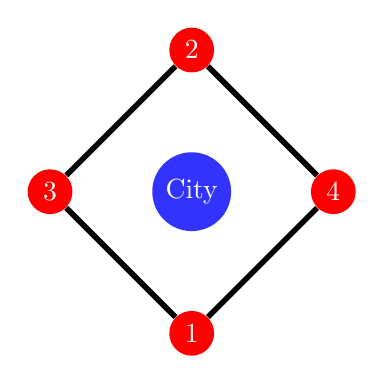
\begin{tikzpicture}
				\node [vertex] (1){City};	
				\node [vertex, fill=red] (2) [below=of 1] {1};
				\node [vertex, fill=red] (3) [above=of 1] {2};
				\node [vertex, fill=red] (4) [left=of 1] {3};
				\node [vertex, fill=red] (5) [right=of 1] {4};
				%edges
				\draw[line width=2pt] (2) -- (5) -- (3) -- (4) -- (2);
				
			\end{tikzpicture}
		\end{column}
	\end{columns}
\end{frame}

\begin{frame}{Consensus}
	\begin{columns}[T]
		\begin{column}{0.49\textwidth}
		{\bf Conditions}
		\begin{enumerate}
			\item All loyal Generals decide upon the same plan of action
			\item A small number of traitors cannot cause the loyal Generals to adopt a bad plan
		\end{enumerate}
		\end{column}
		\begin{column}{0.5\textwidth}
			\begin{itemize}
				\item Traitors can do what they wish
				\item Loyal Generals will all do what they are told
				\item $v(i)$ be information communicated by the $i^{th}$ General. So, you have $v(1),v(2),\ldots,v(n)$, where there are $n$ Generals
			\end{itemize}
		\end{column}
	\end{columns}
\end{frame}

\begin{frame}{Byzantine Generals Problem}{3-node}
	\begin{columns}[T]
		\begin{column}{0.48\textwidth}
		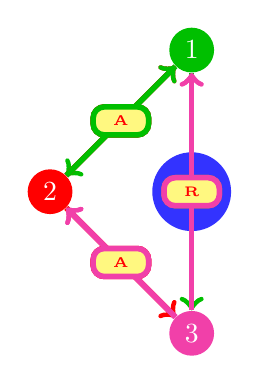
\begin{tikzpicture}
			\node<-1> [vertex] (0){City};
			\node [vertex,fill=red] (2) [left=of 0]{2};
			\node [vertex,fill=green!75!black] (1) [above=of 0]{1};
			\node [vertex,fill=magenta!75!white] (3) [below=of 0]{3};
			%edges
			\draw<3|only@3>(1) edge[Dedge, color=green!75!black] node[label]{A}  (2);
			\draw<3|only@3>(1) edge[Dedge, color=green!75!black] node[label]{A}  (3);
			\draw<3|only@3>(3) edge[Dedge, color=magenta!75!white] node[label]{R} (2);

			\draw<2|only@2> (2) edge[Dedge, color=red] node[label]{A} (3);
			\draw<2|only@2> (2) edge[Dedge, color=red] node[label]{A} (1);
			\draw<2|only@2> (3) edge[Dedge, color=magenta!75!white] node[label]{R} (1);

			\draw<4|only@4>(3)  edge[Dedge, color=magenta!75!white] node[label]{R} (1);
			\draw<4|only@4>(3)  edge[Dedge, color=magenta!75!white] node[label]{A} (2);
			\draw<4|only@4>(2) edge[Dedge, color=green!75!black] node[label]{A} (1);
			
	
		\end{tikzpicture}
		\end{column}
		\begin{column}{0.49\textwidth}
			\begin{itemize}
				\item <-2> 3 nodes, messages `A' and `R' for Attack and Retreat, respectively
				\item <2-> 1 and 2 are loyal; 3 is disloyal. 
				\item <2|only@2> 2 sends the same message to 3 and 1
				\item <2|only@2> 3 changes the message and sends to 1
				\item <2|only@2> 1 receives conflicting messages
				\item <3|only@3> 1 sends the same message
				\item <3|only@3> 3 changes the messages and sends to 2
				\item <3|only@3> 2 receives conflicting messages
				\item <4|only@4> 3 sends different messages to 1 and 2
				\item <4|only@4> 2 forwards the message to 1
				\item <4|only@4> 1 receives conflicting messages
				\item <4-> needs to be $3m+1$, where there are $m$ traitors
				\item <4-> informal proof, formal proof \cite{pease1980reaching}

			\end{itemize}
		\end{column}
	\end{columns}
\end{frame}

\begin{frame}{Byzantine Generals Problem}{4-node}
	\begin{columns}[T]
		\begin{column}{0.48\textwidth}
		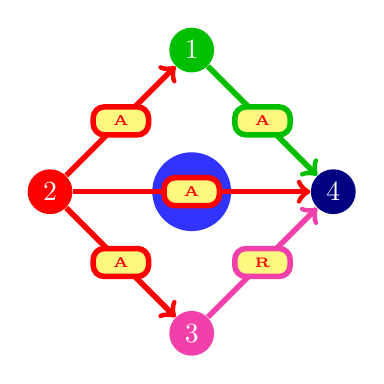
\begin{tikzpicture}
			\node<-1> [vertex] (0){City};
			\node [vertex,fill=red] (2) [left=of 0]{2};
			\node [vertex,fill=green!75!black] (1) [above=of 0]{1};
			\node [vertex,fill=magenta!75!white] (3) [below=of 0]{3};
			\node [vertex,fill=blue!50!black] (4) [right=of 0]{4};
			%edges
%			\draw<3|only@3>(1) edge[Dedge, color=green!75!black] node[label]{A}  (2);
%			\draw<3|only@3>(1) edge[Dedge, color=green!75!black] node[label]{A}  (3);
%			\draw<3|only@3>(3) edge[Dedge, color=magenta!75!white] node[label]{R} (2);
%			\draw<3|only@3>(1) edge[Dedge, color=green!75!black] node[label]{A} (4);
			

			\draw<2|only@2> (2) edge[Dedge, color=red] node[label]{A} (3);
			\draw<2|only@2> (2) edge[Dedge, color=red] node[label]{A} (1);
			\draw<2|only@2> (2) edge[Dedge, color=red] node[label]{A} (4);
			\draw<2|only@2> (1) edge[Dedge, color=green!75!black] node[label]{A} (4);
			\draw<2|only@2> (3) edge[Dedge, color=magenta!75!white] node[label]{R} (4);

%			\draw<4|only@4>(3)  edge[Dedge, color=magenta!75!white] node[label]{R} (1);
%			\draw<4|only@4>(3)  edge[Dedge, color=magenta!75!white] node[label]{A} (2);
%			\draw<4|only@4>(3) edge[Dedge, color=magenta!75!white] node[label]{R} (4);
%			\draw<4|only@4>(2) edge[Dedge, color=green!75!black] node[label]{A} (1);
%			
	
		\end{tikzpicture}
		\end{column}
		\begin{column}{0.49\textwidth}
			\begin{itemize}
				\item <-2> 3 nodes, messages `A' and `R' for Attack and Retreat, respectively
				\item <2-> 1, 2 and 4 are loyal; 3 is disloyal. 
				\item <2|only@2> 2 sends the same message to all nodes 
				\item <2|only@2> 3 changes the message and sends to 4
				\item <2|only@2> 4 receives conflicting messages
				\item <2|only@2> 4 acts on majority of messages 'A'
%				\item <3|only@3> 1 sends the same message to all nodes
%				\item <3|only@3> 3 changes the messages and sends to 2
%				\item <3|only@3> 2 receives conflicting messages
%				\item <4|only@4> 3 sends different messages to 1 and 2
%				\item <4|only@4> 2 forwards the message to 1
%				\item <4|only@4> 1 receives conflicting messages
%				\item <4-> needs to be $3m+1$, where there are $m$ traitors
%				\item <4-> informal proof, formal proof \cite{pease1980reaching}

			\end{itemize}
		\end{column}
	\end{columns}
\end{frame}

\begin{frame}{Practical Byzantium Fault Tolerance (PBFT) \cite{castro1999practical}}
	\begin{itemize}
		\item PBFT was first Byzantium fault tolerant algorithm
		\item PBFT worked in practical and asynchronous environments
		\item leader-based and non-forking
		\item does not support open-enrollment
		\item nodes added by aministrator
		\item requires full P2P
		\item Fault tolerance - preserves liveness and safety
		\item Even when parts of the network are:
			\begin{itemize}
				\item misbehaving
				\item experiencing problems
				\item unconnected
				\item not working properly
				\item behaving dishonestly
			\end{itemize}
		\item Minimum percentage of node in PBFT are?
	\end{itemize}
\end{frame}


\begin{frame}{PBFT? \cite{castro1999practical}}
	\begin{itemize}
		\item cited alot, least understood
		\item \parencite{lamport1982byzantine} 5500+
		\item \parencite{castro1999practical} 2500+
		\item $n$ number of nodes in network
		\item $[0,1,2,3,....,n-2,n-1]$
		\item $f$ Max. bad nodes the network can tolerate 
	\end{itemize}
	\begin{block}{PBFT Equations}
		\begin{equation}
			n=nodes
		\end{equation}
		\begin{equation}
			f=\frac{n-1}{3}
		\end{equation}
		\begin{equation}
			n=3f+1
		\end{equation}
	\end{block}
\end{frame}


\begin{frame}{Voting-based adpated from \cite{sawtooth:consensus}}
	\begin{itemize}
		\item Only a single node can commit
		\item One or more nodes has complete view of network
		\item Adding or removing nodes from the network is difficult
		\item There are many P2P (complete)
	\end{itemize}
\end{frame}

\begin{frame}{PBFT \cite{castro1999practical}}
	\begin{enumerate}
		\item A client send a request to invoke a service operation to the primary
		\item The primary multicasts the request to the backups
		\item Replicas execute the request and send a reply to the client
		\item The client waits for $f+1$ replies from different replicas with the same result; this is the result of the operation
	\end{enumerate}
\end{frame}

\begin{frame}{Problem \cite{sawtooth:consensus}}
	\begin{enumerate}
		\item user sends a message to all the nodes
		\item a series of messages is sent between the nodes to determine if the message is valid
		\item once a number of nodes agree that the request is valid, then the instructions in the request are executed and result is return to client
		\item the client waits for a number of replies that match, then accepts the result
	\end{enumerate}
\end{frame}

\begin{frame}{Definitions}
	\begin{table}
	\rowcolors[]{2}{blue!30}{blue!15}
		\begin{tabular}{p{25mm}p{85mm}}
			{\bf Term } & {\bf Definition}\\
			Node & `Machine' running components necessary to wring a blockchain \\ 
			Server & synonym for Node\\
			Validator & Component of  a node for interactions with the blockchain \\
			Primary & Node in charge \\
			Secondary & Auxillary node used for consensus \\
			Client & `Machine' that sends request and receives replies. \\
			Checkpoint & Point when logs can get garbage collection \\ 
			cp period & How many client requests in between each cp \\
			block duration & block latency \\
			Message & block, with additional information \\
			Working block & block currently being committed, initialised but not finalised \\
			Low water mark & sequence number of the last stable checkpoint\\
			High water mark & low water mark plus the desired maximum size of nodes' message logs\\
			View & scope of PBFT when primary in charge \\
			$n$ & number of nodes \\
			$f$ & max. faulty nodes \\
		\end{tabular}
	\end{table}
\end{frame}

\begin{frame}{Definitions (cont'd)}
	\begin{table}
	\rowcolors[]{2}{blue!30}{blue!15}
		\begin{tabular}{p{25mm}p{85mm}}
			{\bf Term } & {\bf Definition}\\
			Low water mark & sequence number of the last stable checkpoint\\
			High water mark & low water mark plus the desired maximum size of nodes' message logs\\
			View & scope of PBFT when primary in charge \\
			$n$ & number of nodes \\
			$f$ & max. faulty nodes \\
			$v$ & the current view numner \\
			$p$ & primary server number $p=v \mod n$\\
		\end{tabular}
	\end{table}
\end{frame}

\begin{frame}{State Transitions}
	\includegraphics[scale=0.25]{gx/pbft_states}
\end{frame}

\begin{frame}{Proof-of-Work}
	\begin{columns}[T]
		\begin{column}{0.48\textwidth}
			\begin{itemize}
				\item Challenge to solve a very difficult puzzle
				\item Extremely hard to solve 
				\item Very easy to verify correctness of solution
				\item Combination lock
				\item Use of a nonce
			\end{itemize}
		\end{column}
		\begin{column}{0.48\textwidth}
			\begin{block}{PoW}
				\begin{equation}
					H_{a}(d+n) < h
				\end{equation}
				where $H$ is hashing function; $a$ is hashing algorithm (e.g. SHA256); $d$is data; $n$ is nonce; and $h$ is a result of a hashing function usually starting with 4 zeroes.
			\end{block}
		\end{column}
	\end{columns}	
\end{frame}


\begin{frame}{PoW: Example}
	\begin{itemize}
		\scriptsize
		\item $d = 0$
		\item $H(0) =$ 5feceb66ffc86f38d952786c6d696c79c2dbc239dd4e91b46729d73a27fb57e9
		\item target = 	{\bf0}feceb66ffc86f38d952786c6d696c79c2dbc239dd4e91b46729d73a27fb57e9
		\item $n=1$
		\item while ($H(d+n) < target$)
			\begin{itemize}
				\item n++
			\end{itemize}
		\item $H(00x1)=$ 6fbc24c863cad03d71238d38f725383eb79804b1adf05b05511470f18ac66129
		\item $H(00x2)=$ 9eb14f1909e80b0005ea1531e91a315401e5f788e0c5e7f1b7c24f3d2c92e5a4
		\item $H(00x3)=$ 5e847f40960c2fe8fcaf2bf7b11df0cc012f73c59d52cd2ee8f5ee44b2711e85
		\item \vdots
		\item $H(00x48)=$ 0529f9d44d1ec54ce86601d63aac3a094ac90577b175e024058190a6ec062873
		\item target= {\bf 000}ceb66ffc86f38d952786c6d696c79c2dbc239dd4e91b46729d73a27fb57e9
		\item $H(00x80)=$ 00021397ccc9e4e75258c17ac7d651674999ea72c6d3f6dfdae55ca8a2174420
		\normalsize
	\end{itemize}
\end{frame}


\begin{frame}{PoW}
	\begin{itemize}
		\item Waste of Energy
		\item Application-Specific integrated circuit - ASIC
			\begin{itemize}
				\item 1kH/s - 1,000 hashes per second
				\item 1MH/s - 1,000,000 hashes per second
				\item 1GH/s - 1,000,000,000 hashes per second
				\item ASIC chip around 30GH/s
			\end{itemize}
		\item Bitcoin rewards miners
		\item \bitcoinA 50 for firsts 210,000 blocks
		\item \bitcoinA 25 for second 210,000 blocks
		\item \bitcoinA 12 for third 210,000 blocks
		\item No reward? 
			\begin{itemize}
				\item Rely on transaction fees
				\item Less miners and open to 51\% attacks
				\item Change in consensus algorithm?
			\end{itemize}
		\item High latency of TX validation
	\end{itemize}
\end{frame}

\begin{frame}{Proof of Stake}
	\begin{itemize}
		\item Nodes are validators, not miners
		\item Validate a TX, to earn TX fee
		\item Each node has a stake value
		\item Usually, stake cannot be spent
		\item Nodes are selected proportionately to the stake value
		\item Randomness where stakes are equal
		\item Example:
			\begin{itemize}
				\item Node A has 200 MDXCoins
				\item Node B has 100 MDXCoins
				\item Node A is twice as likely to be selected to validate the TX
				\item Upon doing so Node A receives the transaction fee
			\end{itemize}
		\item Many variations on this, Proof-of-Deposit
	\end{itemize}
\end{frame}


\begin{frame}{PoS}
	\begin{columns}[T]
		\begin{column}{0.48\textwidth}
			{\bf Random Selection}
			\begin{itemize}
				\item Ratio between stake:all cryptocurrency
				\item 1\% stake of the entire blockchain results in being selected 1\% of the time
				\item 51\% stake results in 51\% selection
			\end{itemize}
			{\bf Multi-round Voting}
			\begin{itemize}
				\item Byzantine Fault Tolerance PoS \cite{bahsoun2015making}
				\item Select several staked nodes
				\item Staked users cast a vote
				\item Elected creates block
			\end{itemize}
		\end{column}
		\begin{column}{0.48\textwidth}
			{\bf Coin Age}
			\begin{itemize}
				\item Older stakes are more likely to get selected than younger stakes
				\item Age is reset after selection
				\item Fatigue
			\end{itemize}
			{\bf Delegate Systems}
			\begin{itemize}
				\item users vote for nodes to become publishing nodes
				\item voting power is proportionate to stake
				\item incentivised to not act maliciously
				\item rewards and reputation
			\end{itemize}
		\end{column}
	\end{columns}	
\end{frame}



\begin{frame}{PoS}
	\begin{itemize}
		\item Less energy spent
		\item No miners
		\item Does mean bigger stakes, have more probability of being selected
		\item low latency of TX validation
		\item Speeds up block creation
	\end{itemize}
\end{frame}



\begin{frame}{Proof-of-Elapsed-Time, PoET}
	\begin{itemize}
		\item All nodes are validators
		\item Random allocation of wait time
		\item The node with the shortest wait times validates the TX
		\item Permissioned blockchain
		\item Low latency of TX validation
		\item Speeds up block creation \cite{thakkar2018performance}
		\item Does depend on size of block and data in transaction
		\item Scalability is still an issue (50M transactions per second)
	\end{itemize}
\end{frame}



\begin{frame}{Conclusion}
\rowcolors[]{2}{blue!30}{blue!15}
	\begin{tabular}{|l|p{20mm}|p{20mm}|p{20mm}|p{20mm}|p{20mm}|}\hline
		Name & Goals & Advantages & Disadvantages & Domain & Implementation \\ \hline \hline
	\end{tabular}
\end{frame}




\begin{frame}{Summary}
	\begin{table}
		\rowcolors[]{2}{blue!30}{blue!15}
		\begin{tabular}{lllll}
			Criteria & PoW & PoS & Hybrid PoW/S & PoET \\ \hline
			Efficiency & No	& Yes& No & Yes \\
			H/w	 & Very Important & None & Important & None \\ 
			Speed	 & Poor & Good & Poor & Good \\ 
			Example & BitCoin & NextCoin & BlackCoin & HyperLedger \\
		\end{tabular}
	\end{table}
\end{frame}



%\begin{frame}{Enumerator Types}
%	\begin{columns}[T]
%		\begin{column}{0.48\textwidth}
%			\begin{lstlisting}
%			\end{lstlisting}
%		\end{column}
%		\begin{column}{0.48\textwidth}
%			{\bf XXX}
%		\end{column}
%	\end{columns}	
%\end{frame}
%
%

%\begin{frame}{X}
%	\begin{columns}[T]
%		\begin{column}{0.48\textwidth}
%			\begin{itemize}
%				\item XXX 
%			\end{itemize}
%		\end{column}
%		\begin{column}{0.48\textwidth}
%			{\bf XXX}
%		\end{column}
%	\end{columns}	
%\end{frame}

%\begin{frame}{}
%	\begin{itemize}
%		\item
%	\end{itemize}
%\end{frame}


\begin{frame}[allowframebreaks]{References}
	\printbibliography
\end{frame}
	
\end{document}
